% Figure source (posttrain). Rendered to figures/pdf/posttrain.pdf by the
% figure build; delete that PDF to have LaTeX compile this source instead.
% x: fraction of the stage's single epoch (general SFT: 244.1M tokens; task SFT: 28.6M tokens).
% Each stage is validated on its own held-out set, so the two loss levels are not comparable.
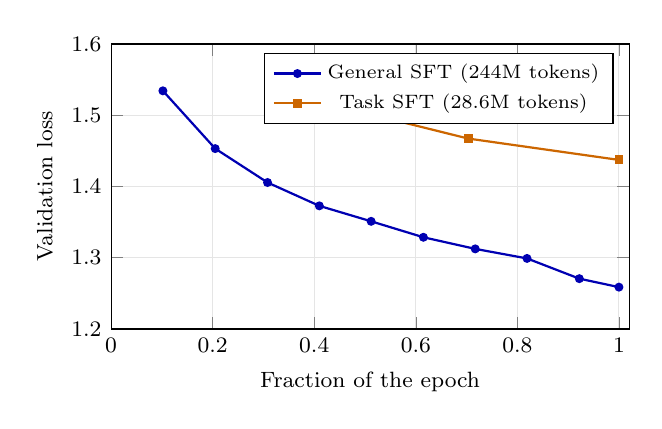
\begin{tikzpicture}
\begin{axis}[
    width=8.16cm, height=5.2cm,
    xlabel={Fraction of the epoch}, ylabel={Validation loss},
    xmin=0, xmax=1.02, ymin=1.2, ymax=1.6,
    tick label style={font=\footnotesize}, label style={font=\footnotesize},
    legend style={font=\scriptsize}, legend pos=north east,
    grid=major, grid style={gray!20}
]
\addplot[blue!70!black, thick, mark=*, mark size=1.2pt] coordinates {
 (0.102,1.5343) (0.205,1.4532) (0.308,1.4056) (0.410,1.3728) (0.512,1.3511) (0.615,1.3287) (0.717,1.3124) (0.819,1.299) (0.922,1.2706) (1.0,1.2587)};
\addlegendentry{General SFT (244M tokens)}
\addplot[orange!80!black, thick, mark=square*, mark size=1.2pt] coordinates {(0.353,1.5293) (0.703,1.4673) (1.0,1.4373)};
\addlegendentry{Task SFT (28.6M tokens)}
\end{axis}
\end{tikzpicture}
